\documentclass[11pt,a4paper,twocolumn]{article}

% === Core Packages ===
\usepackage[margin=2cm]{geometry}
\usepackage[utf8]{inputenc}
\usepackage[T1]{fontenc}
\usepackage{times}
\usepackage{amsmath,amssymb}
\usepackage{graphicx}
\usepackage{booktabs}
\usepackage{float}
\usepackage{enumitem}
\usepackage{tikz}
\usepackage{pgfplots}
\pgfplotsset{compat=1.18}
\usetikzlibrary{arrows.meta,shapes.geometric,positioning,calc,decorations.markings,fit,backgrounds}

% === Citation (IEEE style) ===
\usepackage[numbers,sort&compress]{natbib}
\bibliographystyle{IEEEtranN}

% === Hyperref ===
\usepackage[hidelinks]{hyperref}
\usepackage{xurl}

% === Settings ===
\setlength{\parindent}{1em}
\setlength{\parskip}{0.3em}

% === PDF metadata ===
\hypersetup{
  pdftitle={Decentralizirana reputacijska mreža: Okvir za prirodnu organizaciju društva},
  pdfauthor={Pavel Kudrna},
  pdfsubject={Personix — a decentralized reputation network},
  pdfkeywords={Personix, decentralized reputation, reputation social network,
    decentralized identifiers, DID, meritocracy, censorship resistance},
}

% === Title ===
\title{\textbf{Decentralizirana reputacijska mreža:\\Okvir za prirodnu organizaciju društva}}
\author{Pavel Kudrna\\Personix Project --- \url{https://personix.org}\\Prague, Czechia\\Draft v1 --- March 2026}
\date{}

\begin{document}
\maketitle

% ============================================================
% ABSTRACT
% ============================================================
\begin{abstract}
Osjećaj pravde---uvjerenje da se nepravde ispravljaju i da se zasluge nagrađuju---najsnažnija je kohezivna sila društva. Kada centralizirane institucije upravljanja ne mogu pružiti taj osjećaj jer trošak provođenja prava premašuje vrijednost samog prava, društvena kohezija se raspada. Postojeće institucionalne strukture ne uspijevaju riješiti značajnu klasu sporova na sustavno isti način na koji centralno planiranje ne uspijeva alocirati resurse: kroz asimetriju informacija, nedostatak povratnih petlji i odvojenost donositelja odluka od posljedica njihovih odluka. Ovaj rad predstavlja Reputacijsku društvenu mrežu (RSN): decentralizirani, nepotkupljivi, cenzuri otporni komunikacijski sloj izgrađen na decentraliziranim identifikatorima (DID) koji pseudonimnim sudionicima omogućuje objavljivanje, provjeru i konzumiranje reputacijskih informacija o ponašanju u stvarnom svijetu. Temeljni mehanizam počiva na tri načela dizajna: (1)~asimetričnoj strukturi troškova gdje je čitanje reputacijskih podataka jeftino, ali pisanje zahtijeva provjerljiv napor; (2)~nedeterminističkom protokolu za odabir provjeritelja temeljenom na konzistentnom raspršivanju koji cijenu radikalnih tvrdnji određuje kroz eskalirajuće troškove iteracije; i (3)~tržišno vođenom modelu reputacijskog autoriteta gdje privatni provjeritelji zalažu svoju akumuliranu reputaciju na točnost tvrdnji koje podržavaju. Rezultirajuća arhitektura proizvodi emergentnu meritokraciju bez središnje koordinacije i omogućuje postupan, reverzibilan put migracije od postojećih sustava kojima upravlja država.
\end{abstract}

% ============================================================
% 1. INTRODUCTION
% ============================================================
\section{Uvod}

\subsection{Problem centraliziranog povjerenja}

Suvremeno upravljanje počiva na temeljnoj pretpostavci: da centralizirane institucije mogu posredovati povjerenje između stranaca u velikim razmjerima. Sudovi presuđuju u sporovima. Registri potvrđuju vlasništvo. Regulatorna tijela provode standarde. Te su institucije osmišljene u doba kada su informacije bile oskudne, komunikacija spora, a delegiranje ovlasti središnjem tijelu jedini izvediv mehanizam koordinacije. Centralizirano upravljanje, međutim, zakazuje iz istih strukturnih razloga kao i centralno planiranje: asimetrije informacija, nedostatka povratnih petlji i odvojenosti donositelja odluka od posljedica njihovih odluka.

Pretpostavka zakazuje, primjerice, kada trošak institucionalnog posredovanja premašuje vrijednost spora. Zamislite najmoprimca koji otkrije da unajmljeni stan nema zakonski propisanu potvrdu o električnoj sigurnosti---stanje koje predstavlja neposrednu opasnost za život. Zakonsko pravo najmoprimca da odstupi od ugovora je nedvosmisleno. Ipak, trošak provođenja tog prava putem sudskog sustava premašuje novčanu vrijednost pologa i dugovane štete, čak i uključujući moguću zakonsku naknadu~\cite{czcourtfees}. Racionalan odgovor jest apsorbirati gubitak i izaći.

Ovo nije patološki rubni slučaj. To je zadano iskustvo za značajnu klasu sporova u kojima je šteta stvarna, ali novčani ulozi padaju ispod praga na kojem institucionalno provođenje postaje ekonomski racionalno. Rezultat je sustav koji strukturno pogoduje zlonamjernim akterima: oni koji drugima nanose štetu u obujmu ispod tog praga mogu djelovati nekažnjeno, jer trošak traženja pravde pada na oštećenu stranu.

Gornji primjer preuzet je iz pravnog okruženja autora---češkog sustava građanskog prava. U drugim pravnim tradicijama---običajnom pravu temeljenom na presedanima, običajnom pravu, mješovitim sustavima---pravda zakazuje na različite načine i u različitim stupnjevima, ovisno o kulturnim i procesnim posebnostima jurisdikcije. Čitatelji će vjerojatno prepoznati istovjetne primjere iz vlastitog konteksta. Ono što je strukturno univerzalno jest obrazac: sporovi čija vrijednost pada ispod praga ekonomski racionalnog provođenja završavaju tako da gubitak apsorbira oštećena strana. RSN ne obećava savršenu pravdu---on samo smanjuje strukturnu prednost koju zlonamjerni akteri uživaju kada je institucionalno provođenje neekonomično.

\subsection{Zašto postojeća rješenja ne zadovoljavaju}

\textbf{Okviri decentraliziranog identiteta (DID)}~\cite{did2022} pružaju kriptografske mehanizme za samosuvereno upravljanje identitetom, ali se prvenstveno usredotočuju na provjeru identiteta bez rješavanja šireg pitanja reputacije ponašanja.

\textbf{Soulbound tokeni (SBT)}~\cite{weyl2022} obuhvaćaju uvid da je reputacija neprenosiva, ali se oslanjaju na blockchain infrastrukturu s ograničenjima skalabilnosti i ne bave se ekonomskim poticajima koji upravljaju unosom informacija. Srodni koncepti poput tokena zasluga (npr. Liberland) dijele sličnu filozofiju, ali ostaju vezani za specifične jurisdikcijske okvire.

\textbf{Decentralizirane autonomne organizacije (DAO)}~\cite{buterin2014} provode upravljanje putem pametnih ugovora, ali repliciraju plutokratsku dinamiku u kojoj je utjecaj proporcionalan kapitalu. Kvadratno glasovanje~\cite{buterin2019} to djelomično ublažava, ali ograničava praktičnu primjenu. DAO-i se također suočavaju s temeljnim \emph{problemom proročišta}: pametni ugovori ne mogu pouzdano provjeriti stanja u stvarnom svijetu bez pouzdanog vanjskog izvora, a taj problem nema općenito rješenje unutar blockchain arhitekture.

Nijedan postojeći sustav ne kombinira decentralizaciju, otpornost na cenzuru, pseudonimnost, provjerljiv trošak ulaska i emergentni konsenzus.

\subsection{Doprinosi}

Ovaj rad daje sljedeće doprinose:
\begin{enumerate}[nosep]
\item Definiciju \textbf{Reputacijske društvene mreže (RSN)}, decentraliziranog protokola koji proširuje DID okvir kako bi podržao bilateralnu razmjenu reputacije.
\item \textbf{Nedeterministički protokol za odabir provjeritelja} temeljen na konzistentnom raspršivanju~\cite{karger1997}.
\item \textbf{Načelo skupog radikalizma}, koje cijenu tvrdnji određuje prema njihovoj udaljenosti od mrežnog konsenzusa kroz tri kumulativna kanala troška.
\item \textbf{Model uglednog autoriteta} s asimetričnim poticajima gdje lažno podupiranje košta katastrofalno više od legitimnih naknada.
\item \textbf{Postupan put migracije} kroz paralelnu fiskalnu infrastrukturu.
\end{enumerate}

% ============================================================
% 2. DESIGN PRINCIPLES
% ============================================================
\section{Načela dizajna}

Arhitekturu RSN-a ograničava pet neprekršivih načela dizajna.

\textbf{Kontinuitet i evolucija.} Sustav koegzistira s postojećim institucijama tijekom prijelaznog razdoblja neodređene duljine. Prijelaz mora biti reverzibilan u svakoj fazi.

\textbf{Dobrovoljnost i odgovornost.} Sudjelovanje je dobrovoljno, ali dobrovoljnost je spregnuta s odgovornošću: sudionik koji preuzme kontrolu nad institucionalnom funkcijom istodobno preuzima i pripadajuće obveze.

\textbf{Raznolikost i kulturna neutralnost.} Konsenzus proizlazi iz bilateralnih interakcija, a ne iz unaprijed zadanih pravila koja nameću dizajneri sustava.

\textbf{Otpornost i otpor cenzuri.} Trošak cenzuriranja mreže mora premašiti trošak njezinog toleriranja. Samo potpuni totalitarizam---uz razorne političke i ekonomske troškove---može potisnuti sustav.

\textbf{Konsenzus i provođenje.} Sustav ugrađuje ljudske sklonosti prema sitničavosti, pakosti i osvetničkom zadovoljstvu kao noseće značajke. Nedolično ponašanje nije zabranjeno; ono se naplaćuje.

% ============================================================
% 3. SYSTEM OVERVIEW
% ============================================================
\section{Pregled sustava}

\subsection{Reputacijska društvena mreža}

RSN je decentralizirani komunikacijski sloj ravnopravnih čvorova u kojem sudionici razmjenjuju provjerljive informacije o ponašanju u stvarnom svijetu. Njegova su definirajuća svojstva: decentralizirana i necenzurabilna infrastruktura; pseudonimno sudjelovanje putem DID-ova; asimetrična struktura troškova (čitanje je jeftino, pisanje je skupo); kriptografska provjerljivost; i \textbf{podrška standardima}---strojno čitljivi formati za informacije koje se propagiraju kroz mrežu, za usluge koje nude autoriteti (sastavljanje tvrdnji, podupiranje, usluga svjedočenja) te za format politike uključujući pravila za procjenu reputacije druge strane i procjenu rizika neusklađenosti politike (između deklariranog i stvarnog ponašanja).

\subsection{Arhitektonske komponente}

RSN se sastoji od četiri primarne komponente (Sl.~\ref{fig:architecture}):
\begin{enumerate}[nosep]
\item \textbf{DID sloj.} Identiteti sudionika s deklariranim pravilima, reputacijskim metapodacima i mrežnim usmjeravanjem.
\item \textbf{Protokol tvrdnji.} Strukturirani format za objavljivanje tvrdnji o događajima u stvarnom svijetu.
\item \textbf{Mreža provjere.} Decentralizirani protokol za dodjeljivanje provjeritelja pomoću konzistentnog raspršivanja.
\item \textbf{Sloj agregacije reputacije.} Usluge koje proizvode ljudski čitljive sažetke reputacije.
\end{enumerate}

\begin{figure}[ht]
\centering
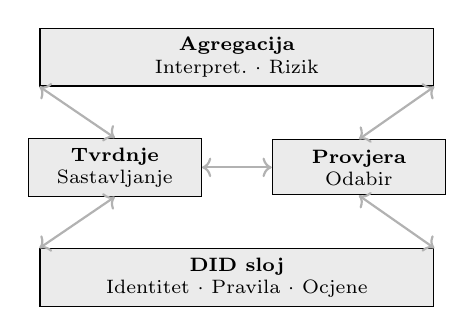
\begin{tikzpicture}[
    layer/.style={draw, minimum height=0.7cm, align=center, font=\scriptsize, fill=black!8},
    arr/.style={<->, thick, gray!60}
]
\node[layer, minimum width=5cm] (agg) at (0,2.8) {\textbf{Agregacija}\\Interpret.\ $\cdot$ Rizik};
\node[layer, minimum width=2.2cm] (claim) at (-1.55,1.4) {\textbf{Tvrdnje}\\Sastavljanje};
\node[layer, minimum width=2.2cm] (verif) at (1.55,1.4) {\textbf{Provjera}\\Odabir};
\node[layer, minimum width=5cm] (did) at (0,0) {\textbf{DID sloj}\\Identitet $\cdot$ Pravila $\cdot$ Ocjene};

\draw[arr] (agg.south west) -- (claim.north);
\draw[arr] (agg.south east) -- (verif.north);
\draw[arr] (claim.east) -- (verif.west);
\draw[arr] (claim.south) -- (did.north west);
\draw[arr] (verif.south) -- (did.north east);
\end{tikzpicture}
\caption{Četveroslojna arhitektura RSN-a.}
\label{fig:architecture}
\end{figure}

\subsection{Uloge sudionika}

Transakcija provjere uključuje do šest različitih DID uloga (Sl.~\ref{fig:roles}): \textbf{Izdavatelj} ($DID_I$, stvara i podnosi tvrdnju), \textbf{Subjekt} ($DID_S$, DID na koji se tvrdnja odnosi---može se podudarati s Izdavateljem), \textbf{Autoritet} ($DID_A$, podupire tvrdnju uz naknadu; može ponuditi i usluge svjedočenja---\emph{neobavezno}), \textbf{Svjedok} ($DID_{W_{1..n}}$, incognito nadzornik poštenja provjeritelja putem izazovnih kodova---\emph{neobavezno}), \textbf{Provjeritelj} ($DID_V$, algoritamski odabran za objavljivanje tvrdnje), i \textbf{RSN} (mreža u kojoj se objavljuju provjerene tvrdnje). Bilo koja uloga može se delegirati drugom DID-u (Odjeljak~7.4). Autoritet obično objedinjuje podupiranje s uslugama svjedočenja, ali su dvije funkcije logički neovisne.

\begin{figure}[ht]
\centering
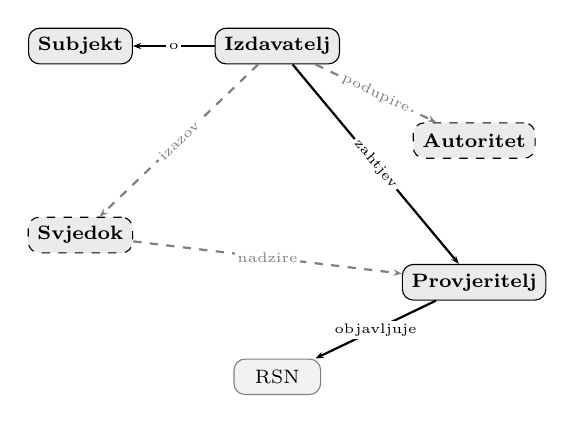
\begin{tikzpicture}[
    role/.style={draw, rounded corners, minimum width=1.1cm, minimum height=0.45cm, align=center, font=\scriptsize, fill=black!8},
    opt/.style={draw, rounded corners, minimum width=1.1cm, minimum height=0.45cm, align=center, font=\scriptsize, fill=black!8, dashed},
    arr/.style={-{Stealth[length=3pt]}, thick},
    oarr/.style={-{Stealth[length=3pt]}, thick, dashed, gray},
    lbl/.style={font=\tiny, fill=white, inner sep=1pt}
]
\node[role] (I) at (0,2.4) {\textbf{Izdavatelj}};
\node[role] (S) at (-2.5,2.4) {\textbf{Subjekt}};
\node[opt] (A) at (2.5,1.2) {\textbf{Autoritet}};
\node[opt] (W) at (-2.5,0) {\textbf{Svjedok}};
\node[role] (V) at (2.5,-0.6) {\textbf{Provjeritelj}};
\node[role, fill=black!5, draw=gray] (N) at (0,-1.8) {RSN};

\draw[arr] (I) -- node[lbl] {o} (S);
\draw[oarr] (I) -- node[lbl,sloped] {podupire} (A);
\draw[oarr] (I) -- node[lbl,sloped] {izazov} (W);
\draw[arr] (I) -- node[lbl,sloped] {zahtjev} (V);
\draw[oarr] (W) -- node[lbl] {nadzire} (V);
\draw[arr] (V) -- node[lbl] {objavljuje} (N);
\end{tikzpicture}
\caption{DID uloge u transakciji provjere. Iscrtkano = neobavezno (Autoritet, Svjedok).}
\label{fig:roles}
\end{figure}

\subsection{Nepotkupljivost: četiri sile}

Nepotkupljivost RSN-a ne proizlazi iz jednog mehanizma, već iz četiri istodobne sile. Nijedna nije sama po sebi dovoljna; tek njihova kombinacija čini pokušaj korupcije ekonomski iracionalnim.

\textbf{Nepredvidljiva meta.} Provjeritelj za svaku tvrdnju odabire se nedeterministički putem konzistentnog raspršivanja (Odjeljak~5.3). Napadač ne može unaprijed ciljati određenog provjeritelja radi podmićivanja, jer je identitet provjeritelja funkcija sadržaja tvrdnje i prethodnih iteracija, a ne izbora izdavatelja.

\textbf{Reputacijska poluga---sporo gore, brzo dolje.} Reputacija se može steći samo postupno, kroz dugotrajno dosljedno ponašanje. Međutim, može se katastrofalno izgubiti jednim prijevarnim podupiranjem (Odjeljak~6.2). Ta asimetrija znači da se godine akumulirane reputacije mogu uništiti jednim nepoštenim podupiranjem; optimalna strategija ostaje odbijanje sumnjivih tvrdnji.

\textbf{Javno obećanje.} Svaki nositelj DID-a javno deklarira svoju politiku---strojno čitljiv skup pravila kojih se obvezuje pridržavati. Razilaženje između deklaracije i stvarnog ponašanja je otkrivo i naplaćuje se kao reputacijski prekršaj teži od samog kršenja (Odjeljak~7.3). Licemjerje je stoga skuplje od izravne nepoštenosti.

\textbf{Asimetrija troška napada na mrežu.} Trošak cenzuriranja ili destabilizacije mreže raste nelinearno s veličinom i gustoćom mreže, dok trošak njezinog toleriranja ostaje konstantan. Da bi se cenzura isplatila, centralizirani bi je akter morao primijeniti na cijelu mrežu---što zahtijeva mjere nesrazmjerne bilo kojoj zamislivoj koristi (Odjeljak~10).

% ============================================================
% 4. DECENTRALIZED IDENTITY MODEL
% ============================================================
\section{Model decentraliziranog identiteta}

\subsection{DID s posebnim svojstvima}

RSN proširuje W3C DID Core specifikaciju~\cite{did2022} sa: \textbf{deklariranim pravilima} (strojno čitljive obveze ponašanja), \textbf{reputacijskim metapodacima} (agregirana ocjena ponašanja) i \textbf{mrežnim usmjeravanjem} (promjenjivi onion pristupnik odvojen od stabilne pozicije na prstenu).

\subsection{Životni ciklus tvrdnje}

Tvrdnja prolazi kroz šest faza (Sl.~\ref{fig:lifecycle}): sastavljanje, neobavezno podupiranje autoriteta, odabir provjeritelja putem konzistentnog raspršivanja, odluka o provjeri (prihvaćanje ili odbijanje s iteracijom), objava i ažuriranje reputacije za sve strane.

\begin{figure}[ht]
\centering
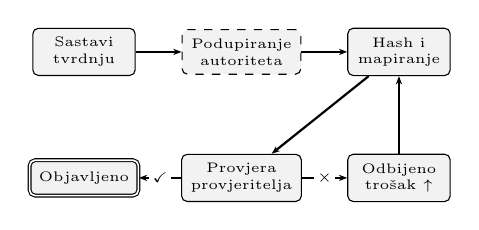
\begin{tikzpicture}[
    stp/.style={draw, rounded corners=2pt, minimum width=1.3cm, minimum height=0.45cm, align=center, font=\tiny, fill=black!5},
    arr/.style={-{Stealth[length=3pt]}, thick},
    lbl/.style={font=\tiny, fill=white, inner sep=1pt}
]
\node[stp] (comp) at (0,0) {Sastavi\\tvrdnju};
\node[stp, dashed] (auth) at (2.0,0) {Podupiranje\\autoriteta};
\node[stp] (hash) at (4.0,0) {Hash i\\mapiranje};
\node[stp] (ver) at (2.0,-1.6) {Provjera\\provjeritelja};
\node[stp, double] (pub) at (0,-1.6) {Objavljeno};
\node[stp] (rej) at (4.0,-1.6) {Odbijeno\\trošak $\uparrow$};

\draw[arr] (comp) -- (auth);
\draw[arr] (auth) -- (hash);
\draw[arr] (hash) -- (ver);
\draw[arr] (ver) -- node[lbl] {\checkmark} (pub);
\draw[arr] (ver) -- node[lbl] {$\times$} (rej);
\draw[arr] (rej) -- ++(0,0.8) -| (hash);
\end{tikzpicture}
\caption{Životni ciklus tvrdnje s petljom iteracije.}
\label{fig:lifecycle}
\end{figure}

\subsection{Odnos prema W3C DID Core}

Model identiteta RSN-a pravi je nadskup W3C DID Core specifikacije~\cite{did2022}. Svi RSN DID-ovi su valjani W3C DID-ovi. Proširenja specifična za RSN kodirana su kao svojstva DID dokumenta definirana u namjenskoj specifikaciji DID metode, kompatibilnoj s postojećom infrastrukturom poput ION-a~\cite{buchner2021} i Ceramica~\cite{ceramic2023}.

% ============================================================
% 5. VERIFICATION AND PROPAGATION
% ============================================================
\section{Provjera i propagacija informacija}

\subsection{Trošak unosa informacija}

Temeljno ekonomsko načelo RSN-a jest asimetrija između čitanja i pisanja. Čitanje reputacijskih podataka približava se nultom graničnom trošku za sudionike koji su dio DID mreže i imaju pristup razmjeran svojoj reputaciji---pridošlice moraju postupno zaraditi širi pristup (vidi anti-parazitizam). Pisanje---shvaćeno kao trajna materijalizacija reputacije u mreži, a ne kao jednokratni tehnički čin---zahtijeva provjerljivo kumulativno ulaganje kroz tri dimenzije: \textbf{vrijeme} (godine života provedene u dosljednom ponašanju, ispunjenim obvezama i njegovanim odnosima), \textbf{energiju} (napor uložen u pošteno postupanje, brigu o partnerstvima i dugoročnu pouzdanost) i \textbf{novac} (ulaganje u vlastito ime---profesionalni razvoj, kvaliteta vlastitog rada, naknada za nanesene štete). Reputacija se ne može trenutno kupiti---ona je ishod cjeloživotne akumulacije koju sustav samo čini vidljivom i prenosivom kroz kontekste. Jednokratni tehnički troškovi protokola (kriptografski potpisi, naknade provjeritelja) zanemarivi su u usporedbi s tim temeljnim ulaganjem.

\subsection{Društveni graf i dubina kontakata}

RSN je u osnovi društvena mreža: svaki DID dodaje kontakte (druge DID-ove) koji dopuštaju povezivanje. Ti kontakti imaju vlastite kontakte, i tako dalje. Algoritamsko pretraživanje provjeritelja djeluje unutar podesive dubine $h$ povezanih kontakata (npr. $h=3$: vlastiti izravni kontakti, njihovi kontakti i kontakti kontakata). Ova arhitektura ne zahtijeva jedinstveni globalni blockchain---ona prirodno pogoduje pojavi zajednica/klastera s preklapanjima u druge zajednice. Svaki DID sudionik mora imati objavljenu \textbf{politiku}---strojno čitljiv skup pravila koja upravljaju načinom vrednovanja dolaznih zahtjeva. Kršenja politike bilježe se u mreži kao negativni artefakti.

\subsection{Algoritamski odabir provjeritelja}

Protokol provjere koristi konzistentno raspršivanje~\cite{karger1997} (Sl.~\ref{fig:verifier}). Provjera je plaćena usluga: provjeritelji djeluju uz naknadu, stvarajući tržište na kojem konkurencija oblikuje cijene, brzinu i pouzdanost.

\textbf{Korak 1.} Dokument tvrdnje se spaja s rezultatom raspršivanja prethodne iteracije (ili $\varnothing$ u prvoj iteraciji) i raspršuje:
\begin{equation}
\text{pos} = f_h(\text{claim} \| \text{prev\_hash})
\label{eq:hash}
\end{equation}

Algoritam mora uključivati \emph{cjelovit put} svih prethodnih zahtjeva i odgovora---ne samo hash prethodne iteracije. Cjeloviti odgovor svakog provjeritelja (prihvaćanje, odbijanje, ponuđena cijena, razlog) dodaje se rastućem dokumentu, provjerljiv putem kriptografskih potpisa u svakom koraku.

\textbf{Korak 2.} Hash se mapira na $N$ pozicija na prstenu konzistentnog raspršivanja, ravnomjerno raspoređenih (npr. za $N=4$: $+0^{\circ}, +90^{\circ}, +180^{\circ}, +270^{\circ}$). Iz svake pozicije, pretraga u smjeru kazaljke na satu odabire najbliži DID kao kandidata za provjeritelja (Sl.~\ref{fig:multipoint}). $N$ je varijabilan parametar koji može ovisiti o postotku trenutno aktivnih DID-ova, dobu dana ili povijesnoj odzivnosti mreže.

\textbf{Korak 3.} Provjeritelj prihvaća (objavljuje, zalažući reputaciju) ili odbija (vraćajući se na Korak~1 s hashom odbijanja). Kada čvor ne odgovori unatoč deklariranom statusu online, sljedeći zahtjev mora uključivati sve odgovore od svih $N$ prethodnih kandidata za provjeritelja.

\textbf{Anti-parazitizam.} Ciljni DID-ovi mogu postaviti naknade ili ograničenja pristupa za upite od novih DID-ova s malo reputacije. Taj postupni mehanizam (ne binarni) prisiljava pridošlice da izgrade reputaciju kroz istinsku aktivnost prije nego što slobodno konzumiraju tuđe podatke.

\begin{figure}[ht]
\centering
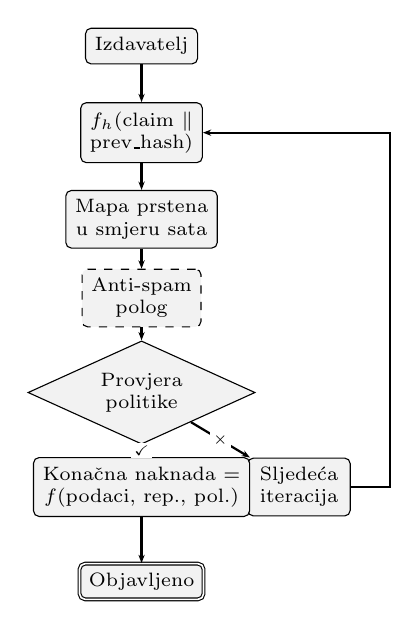
\begin{tikzpicture}[
    box/.style={draw, rounded corners=2pt, minimum width=1.3cm, minimum height=0.45cm, align=center, font=\scriptsize, fill=black!5},
    dec/.style={draw, diamond, aspect=2.2, minimum width=0.9cm, align=center, font=\scriptsize, fill=black!5},
    arr/.style={-{Stealth[length=3pt]}, thick},
    lbl/.style={font=\tiny, fill=white, inner sep=1pt}
]
\node[box] (iss) at (0,0) {Izdavatelj};
\node[box] (hash) at (0,-1.1) {$f_h$(claim $\|$\\prev\_hash)};
\node[box] (ring) at (0,-2.2) {Mapa prstena\\u smjeru sata};
\node[box, dashed] (spam) at (0,-3.2) {Anti-spam\\polog};
\node[dec] (check) at (0,-4.4) {Provjera\\politike};
\node[box] (rej) at (2,-5.6) {Sljedeća\\iteracija};
\node[box] (fee) at (0,-5.6) {Konačna naknada =\\$f$(podaci, rep., pol.)};
\node[box, double] (pub) at (0,-6.8) {Objavljeno};

\draw[arr] (iss) -- (hash);
\draw[arr] (hash) -- (ring);
\draw[arr] (ring) -- (spam);
\draw[arr] (spam) -- (check);
\draw[arr] (check) -- node[lbl] {$\times$} (rej);
\draw[arr] (check) -- node[lbl] {\checkmark} (fee);
\draw[arr] (fee) -- (pub);
\draw[arr] (rej.east) -- ++(0.5,0) |- (hash.east);
\end{tikzpicture}
\caption{Protokol odabira provjeritelja. Anti-spam polog je neobavezan i može biti povratan. Konačna naknada plaća se samo pri prihvaćanju.}
\label{fig:verifier}
\end{figure}

Svako odbijanje dodaje cjeloviti odgovor provjeritelja (uključujući razloge i uvjete) dokumentu tvrdnje, proširujući njegov sadržaj. Iz proširenog dokumenta nedeterministički se izračunava novi hash, mapirajući na drugu poziciju prstena i odabirući drugog provjeritelja. Dokumentiranje cjelovitog puta je obavezno---izdavatelj ne može predvidjeti ni utjecati na sljedećeg provjeritelja. Ako provjeritelj zanemari zahtjev unatoč kompatibilnoj deklariranoj politici, svjedoci (ako su prisutni) to bilježe, a izdavatelj može priložiti dokaze svjedoka pri konačnoj objavi.

\begin{figure}[ht]
\centering
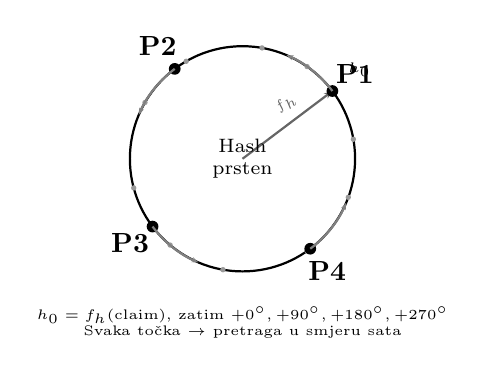
\begin{tikzpicture}[scale=0.65]
% Ring
\draw[thick] (0,0) circle (2.2cm);
% DID nodes on ring
\foreach \a in {10,55,80,120,150,195,230,260,305,340} {
  \fill[black!40] (\a:2.2) circle (1.5pt);
}
% Hash offset arrow pointing to initial position
\draw[-{Stealth[length=3pt]}, thick, black!60] (0,0) -- node[font=\tiny,above,sloped,pos=0.6] {$f_h$} (37:2.2);
\fill[black] (37:2.2) circle (2pt);
\node[font=\tiny,anchor=south west] at (37:2.35) {$h_0$};
% N=4 points offset from h0 by +0, +90, +180, +270
\foreach \offset/\l in {0/P1,90/P2,180/P3,270/P4} {
  \pgfmathsetmacro{\ang}{37+\offset}
  \node[fill=black, circle, inner sep=1.5pt] (p\offset) at (\ang:2.2) {};
  \node[font=\tiny,font=\bfseries] at (\ang:2.75) {\l};
  % clockwise search arc
  \draw[-{Stealth[length=2.5pt]}, thick, gray] (\ang:2.2) arc (\ang:\ang+30:2.2);
}
\node[font=\scriptsize, align=center] at (0,0) {Hash\\prsten};
\node[font=\tiny, align=center] at (0,-3.2) {$h_0 = f_h(\text{claim})$, zatim $+0^{\circ},+90^{\circ},+180^{\circ},+270^{\circ}$\\Svaka točka $\rightarrow$ pretraga u smjeru sata};
\end{tikzpicture}
\caption{Višetočkovni odabir ($N{=}4$). Hash $h_0$ postavlja pomak; 4 točke ravnomjerno raspoređene od $h_0$.}
\label{fig:multipoint}
\end{figure}

\subsection{Protokol svjedoka}

Uloga \textbf{Svjedoka} pruža incognito odgovornost za poštenje provjeritelja kroz kriptografski protokol izazovnog koda:

\textbf{Korak W1.} Podnositelj zahtjeva potpisuje zahtjev za provjeru i šalje ga $N_w$ svjedocima---kontaktima iz podnositeljeve društvene mreže, ili specijaliziranim pružateljima usluge svjedočenja koji djeluju uz naknadu.

\textbf{Korak W2.} Svaki svjedok $w_i$ potpisuje cjeloviti potpisani zahtjev, zadržava izvorni potpis $\sigma_i$ i izračunava izazovni kod $c_i = h(\sigma_i)$. Izazovni kod dodaje se zahtjevu.

\textbf{Korak W3.} Zahtjev, koji sada nosi $N_w$ izazovnih kodova, šalje se provjeritelju. Provjeritelj vidi kodove, ali \emph{ne može utvrditi} tko su svjedoci ni odgovaraju li kodovi stvarnim potpisima.

\textbf{Korak W4 (pošten provjeritelj).} Ako provjeritelj odgovori u skladu sa svojom deklariranom politikom, izazovni kodovi ostaju neprozirni. Svjedoci se nikada ne otkrivaju. Nikakvi dodatni podaci se ne objavljuju.

\textbf{Korak W5 (kršenje politike).} Ako provjeritelj prekrši svoju politiku (zanemari zahtjev, odgovori nedosljedno), podnositelj zahtjeva drži izvorne potpise svjedoka $\sigma_i$. Oni se mogu objaviti kao popratni podaci: svatko može provjeriti $c_i = h(\sigma_i)$, dokazujući da je svjedok bio prisutan. Podnositelj zahtjeva može objaviti neovisno---provjeritelj je već potpisao izazovne kodove u svom odgovoru.

\textbf{Svojstvo blefa.} Podnositelj zahtjeva može zamijeniti neke ili sve izazovne kodove nasumičnim vrijednostima. Provjeritelj ne može razlikovati istinske kodove (potkrijepljene visokoreputiranim autoritetima) od šuma. Ta \emph{neizvjesnost} je mehanizam provođenja: svaki zahtjev nosi rizik da ugledni autoritet promatra incognito. Trošak održavanja tog pritiska gotovo je nula (generiranje nasumičnih brojeva), dok je potencijalni trošak nepoštenja za provjeritelja katastrofalan. Pošteno ponašanje potiče se čak i u odsutnosti stvarnih svjedoka.

\textbf{Autoritet kao svjedok.} Autoritet koji podupire tvrdnju može objediniti usluge svjedočenja: ,,Podupirem vašu tvrdnju i služim kao incognito svjedok tijekom provjere.'' To je prirodan poslovni model---autoritet već ima kontekst. Međutim, dvije su uloge logički neovisne.

\subsection{Načelo skupog radikalizma}

Tri kanala troška zbrajaju se istodobno (Sl.~\ref{fig:radicalism}):

\textbf{Kanal 1: Trošak iteracije.} Svako odbijanje prisiljava na novu iteraciju koja troši vrijeme i resurse. Linearni rast.

\textbf{Kanal 2: Bujanje dokumenta.} Svaka iteracija dodaje cjeloviti odgovor provjeritelja dokumentu tvrdnje. Rast je linearan, ali s osnovnim pomakom: početni sadržaj (sadržaj tvrdnje, podupiranje autoriteta, kriptografski potpisi) već ima netrivijalnu veličinu $B_0$. Ukupna veličina nakon $k$ iteracija: $S(k) = B_0 + k \cdot \Delta$, gdje je $\Delta$ prosječna veličina odgovora.

\textbf{Kanal 3: Premija za rizik provjeritelja.} Rizik je subjektivan. Provjeritelj procjenjuje jesu li deklarirane politike DID-a koji podnosi zahtjev u sukobu s provjeriteljevim vlastitim komercijalnim, društvenim ili političkim interesima. Premija može eksponencijalno eskalirati s percipiranom udaljenošću od provjeriteljevog ,,ideala'': $P(d) = \alpha \cdot e^{\beta d}$, gdje je $d$ provjeriteljeva subjektivna mjera udaljenosti. Iza osobne granice odbijanja, provjeritelj može u potpunosti odbiti.

\begin{figure}[ht]
\centering
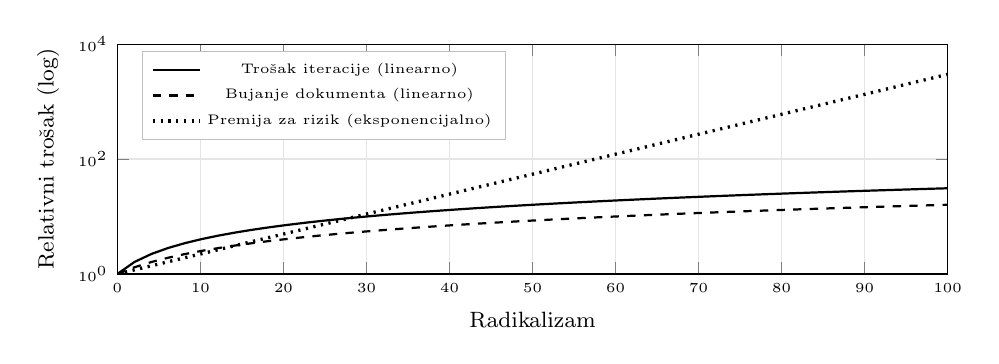
\begin{tikzpicture}
\begin{axis}[
    width=\columnwidth,
    height=4.5cm,
    xlabel={\footnotesize Radikalizam},
    ylabel={\footnotesize Relativni trošak (log)},
    ymode=log,
    xmin=0, xmax=100,
    ymin=1, ymax=10000,
    grid=major,
    grid style={gray!20},
    legend style={at={(0.03,0.97)},anchor=north west,font=\tiny,draw=gray!50},
    tick label style={font=\tiny},
    label style={font=\footnotesize},
]
\addplot[black, thick, domain=0:100, samples=50] {1 + 0.3*x};
\addlegendentry{Trošak iteracije (linearno)}
\addplot[black, thick, dashed, domain=0:100, samples=50] {1 + 0.15*x};
\addlegendentry{Bujanje dokumenta (linearno)}
\addplot[black, thick, dotted, line width=1.2pt, domain=0:100, samples=100] {exp(0.08*x)};
\addlegendentry{Premija za rizik (eksponencijalno)}
\end{axis}
\end{tikzpicture}
\caption{Eskalacija troška kroz tri kanala. Premija za rizik dominira pri visokom radikalizmu.}
\label{fig:radicalism}
\end{figure}

Ključno, ovo nije cenzura. Nijedna tvrdnja nije zabranjena. Sustav naplaćuje rizik (Tablica~\ref{tab:costs}).

\begin{table}[ht]
\centering
\caption{Usporedba troškova po vrstama tvrdnji.}
\label{tab:costs}
\footnotesize
\begin{tabular}{@{}lcccc@{}}
\toprule
\textbf{Vrsta} & \textbf{Iter.} & \textbf{Dok.} & \textbf{Nakn.} & \textbf{Ukupno} \\
\midrule
Vjerodostojna & $k_{\min}$ & $B_0$ & $P_{\min}$ & Nizak \\
Kontroverzna & $k_{\text{med}}$ & $B_0{+}k\Delta$ & $\alpha e^{\beta d}$ & Umjeren \\
Radikalna & $k_{\max}$ & $\gg B_0$ & $\gg P_{\min}$ & Vrlo visok \\
Prijevarna & $\to\infty$ & --- & --- & Neobjavljiva \\
\bottomrule
\end{tabular}
\end{table}

% ============================================================
% 6. REPUTATION AND RISK
% ============================================================
\section{Procjena reputacije i rizika}

\subsection{Model akumulacije reputacije}

Reputacija pokazuje tri svojstva: \textbf{sporu akumulaciju} (postupni rast kroz dosljedno ponašanje), \textbf{brzo uništenje} (jedna prijevara može katastrofalno smanjiti ocjenu) i \textbf{individualno vrednovanje} (svaka konzumirajuća strana može primijeniti vlastitu funkciju agregacije).

\subsection{Ugledni autoriteti}

Ugledni autoritet pregledava tvrdnje i, ako je zadovoljan, supotpisuje ih---zalažući vlastitu reputaciju (Sl.~\ref{fig:authority}). Asimetrija je namjerna: stjecanje reputacije je sporo (postupno $+\delta$ po poštenom podupiranju), dok je njezin gubitak katastrofalan ($-\Delta \gg \delta$ po lažnom podupiranju; ilustrativno, npr. $+2\%$ nasuprot $-70\%$). Optimalna strategija uvijek je odbiti sumnjive tvrdnje. Konkretne vrijednosti $\delta$ i $\Delta$ su parametri sustava.

\begin{figure}[ht]
\centering
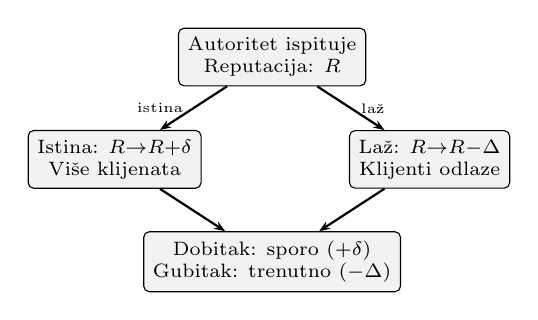
\begin{tikzpicture}[
    box/.style={draw, rounded corners=2pt, minimum width=2cm, minimum height=0.6cm, align=center, font=\scriptsize, fill=black!5},
    arr/.style={-{Stealth[length=4pt]}, thick}
]
\node[box] (exam) at (0,0) {Autoritet ispituje\\Reputacija: $R$};
\node[box] (true) at (-2,-1.3) {Istina: $R{\to}R{+}\delta$\\Više klijenata};
\node[box] (false) at (2,-1.3) {Laž: $R{\to}R{-}\Delta$\\Klijenti odlaze};
\node[box] (insight) at (0,-2.6) {Dobitak: sporo ($+\delta$)\\Gubitak: trenutno ($-\Delta$)};

\draw[arr] (exam) -- node[left,font=\tiny] {istina} (true);
\draw[arr] (exam) -- node[right,font=\tiny] {laž} (false);
\draw[arr] (true) -- (insight);
\draw[arr] (false) -- (insight);
\end{tikzpicture}
\caption{Ugledni autoritet---asimetrični poticaji.}
\label{fig:authority}
\end{figure}

\subsection{Višedimenzionalna reputacija}

Reputacija nije skalar, već vektor kroz više dimenzija: financijska pouzdanost, osobni integritet, profesionalna kompetencija, građanski angažman i druge (Sl.~\ref{fig:reputation-radar}). Različiti pružatelji vrednovanja projiciraju ovaj vektor drugačije ovisno o kontekstu---zajmodavac prioritizira financijsku pouzdanost, poslodavac profesionalnu kompetenciju, susjed građansko ponašanje. Ne postoji jedinstvena ,,ispravna'' ocjena reputacije; samo perspektive.

\begin{figure}[ht]
\centering
\begin{tikzpicture}[scale=0.55]
\foreach \a/\l in {90/Financijska,162/Integritet,234/Profesionalna,306/Građanska,18/Društvena} {
  \draw[gray!40] (0,0) -- (\a:2.5);
  \node[font=\tiny, align=center] at (\a:3.1) {\l};
  \foreach \r in {0.8,1.6,2.4} {
    \fill[black!15] (\a:\r) circle (0.5pt);
  }
}
\draw[thick, fill=black!10] (90:2.0) -- (162:1.2) -- (234:1.8) -- (306:0.9) -- (18:1.5) -- cycle;
\draw[thick, dashed] (90:1.4) -- (162:2.1) -- (234:0.8) -- (306:2.0) -- (18:1.1) -- cycle;
\node[font=\tiny] at (0,-3.3) {Puna: DID A \quad Iscrtkana: DID B};
\end{tikzpicture}
\caption{Višedimenzionalni vektori reputacije. Različiti DID-ovi pokazuju različite profile kroz dimenzije.}
\label{fig:reputation-radar}
\end{figure}

\subsection{Demokratizirana procjena rizika}

RSN demokratizira sustavnu procjenu rizika---sposobnost trenutno koncentriranu u financijskim institucijama, ali primjenjivu daleko izvan bankarstva. Industrijski konglomerati koji procjenjuju pouzdanost dobavljača, osiguravajuća društva koja određuju cijenu bihevioralnog rizika, dubinska analiza za spajanja i preuzimanja, procjena životnog vijeka opreme u proizvodnji---gdje god rizik druge strane zahtijeva procjenu, RSN pruža decentraliziranu, tržišno vođenu alternativu. Tržište usluga interpretacije prevodi sirove višedimenzionalne reputacijske podatke u upotrebljive sažetke, čineći vrednovanje druge strane dostupnim svakom sudioniku uz granični trošak.

% ============================================================
% 7. CONSENSUS AND DISPUTE RESOLUTION
% ============================================================
\section{Konsenzus i rješavanje sporova}

\subsection{Model decentralizirane pravde}

RSN preoblikuje pravdu kao problem bilateralnog pregovaranja. Prijetnja trajnom, provjerljivom štetom po reputaciji učinkovitiji je odvraćajući čimbenik od sudskih postupaka koje oštećena strana ne može priuštiti.

\subsection{Emergentni konsenzus}

Svaki sudionik održava osobni prag zadovoljstva. Agregatni konsenzus mreže pojavljuje se kao statistički prosjek tisuća bilateralnih pregovora (Sl.~\ref{fig:consensus}). Odgovor daleko iznad konsenzusa (barbarski) skup je za objavu. Odgovor blizu konsenzusa (proporcionalan) je jeftin. Konsenzus nije pravilo---on je cjenovni signal.

\begin{figure}[ht]
\centering
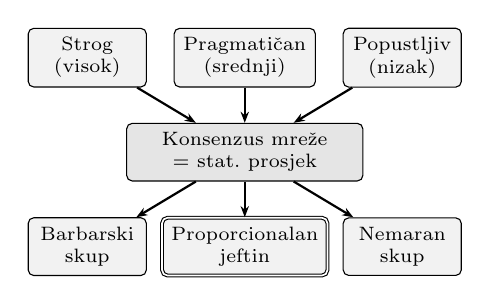
\begin{tikzpicture}[
    person/.style={draw, rounded corners=2pt, minimum width=1.5cm, minimum height=0.5cm, align=center, font=\scriptsize, fill=black!5},
    arr/.style={-{Stealth[length=4pt]}, thick}
]
\node[person] (a) at (-2,0) {Strog\\(visok)};
\node[person] (b) at (0,0) {Pragmatičan\\(srednji)};
\node[person] (c) at (2,0) {Popustljiv\\(nizak)};
\node[person, fill=black!10, minimum width=3cm] (cons) at (0,-1.2) {Konsenzus mreže\\= stat.\ prosjek};
\node[person] (exp) at (-2,-2.4) {Barbarski\\skup};
\node[person, double] (prop) at (0,-2.4) {Proporcionalan\\jeftin};
\node[person] (neg) at (2,-2.4) {Nemaran\\skup};

\draw[arr] (a) -- (cons);
\draw[arr] (b) -- (cons);
\draw[arr] (c) -- (cons);
\draw[arr] (cons) -- (exp);
\draw[arr] (cons) -- (prop);
\draw[arr] (cons) -- (neg);
\end{tikzpicture}
\caption{Emergentni konsenzus iz individualnih pragova zadovoljstva.}
\label{fig:consensus}
\end{figure}

\subsection{Kalibracija kazne}

Svaki nositelj DID-a javno deklarira odgovore na specifične kategorije nedoličnog ponašanja. Nesrazmjerno stroge ili blage deklaracije privlače negativne reputacijske signale. Proporcionalne deklaracije prihvaćaju se bez trvenja---samokalibrirajući sustav kažnjavanja.

Deklaracije konsenzusa i same podliježu otkrivanju licemjerja: deklarativno obvezivanje na konsenzusnu poziciju uz nedosljedno ponašanje predstavlja reputacijski prekršaj teži od samog odstupanja, jer pokazuje namjernu prijevaru.

\subsection{Delegiranje}

Sve aktivnosti unutar DID-a---uz jednu iznimku---mogu se delegirati drugom DID-u. \textbf{Uloga Subjekta---DID-a čije je ponašanje predmet tvrdnje---ne može se delegirati; ona je neprenosivo vezana za nositelja identiteta na kojeg se tvrdnja odnosi.} Ostale aktivne uloge---Izdavatelj, Autoritet, Svjedok, Provjeritelj---mogu se prenijeti na određeni delegatski DID, bilo za provjeru, podnošenje tvrdnji, sudjelovanje u konsenzusu ili rješavanje sporova. Delegiranje je opozivo u svakom trenutku. To omogućuje specijalizaciju (npr. profesionalne usluge provjere) dok nositelj zadržava krajnju kontrolu i odgovornost. Delegiranje se primjenjuje na cijeli sustav i ključno je za skalabilnost.

\subsection{Od individualnog morala do emergentnog društvenog ugovora}

Deklarirana politika svakog DID-a predstavlja formalizaciju individualnog morala: što nositelj smatra prihvatljivim, kako reagira na specifična ponašanja, što zahtijeva od drugih strana. Te politike ne nameće dizajner sustava---bira ih svaki sudionik i izražava u strojno čitljivom obliku.

Ta formalizacija omogućuje trostupanjsku emergenciju. Prvo, individualni moral kodiran je kao \textbf{politika}---skup deklariranih pravila, pragova i funkcija odgovora kojih se DID obvezuje pridržavati. Drugo, agregat svih politika kroz mrežu proizvodi \textbf{emergentnu etiku}---statistički vidljive norme koje nijedan pojedini sudionik nije osmislio, ali koje proizlaze iz interakcije tisuća individualnih moralnih pozicija~\cite{durkheim1893}. Treće, ta emergentna etika, izražena kao zajedničke norme ponašanja provođene kroz bilateralne cjenovne signale, čini \textbf{mjerljiv društveni ugovor}---ne teorijski konstrukt koji nitko nije potpisao~\cite{rawls1971}, već empirijski uočljiv skup pravila potkrijepljen stvarnim ponašanjem.

Taj proces zrcali nalaze teorije moralnih temelja~\cite{haidt2012}: ljudski moral je intuitivan, pluralistički i kulturno varijabilan. RSN ne zahtijeva moralni konsenzus kao ulaz; on proizvodi bihevioralni konsenzus kao izlaz. Rezultirajući društveni ugovor nije statičan---on se razvija kako se sudionici pridružuju, odlaze i prilagođavaju svoje politike kao odgovor na povratne informacije mreže. Za razliku od klasične teorije društvenog ugovora, ovaj ugovor je opoziv, uočljiv i provediv bez suverena.

% ============================================================
% 8. ECONOMIC MODEL
% ============================================================
\section{Ekonomski model}

Prethodni odjeljci opisali su alat---mehanizme provjere RSN-a, strukturu troškova i emergentni konsenzus. Ovaj odjeljak opisuje metodologiju za primjenu tog alata na fiskalnu i upravljačku tranziciju. Alat je opće namjene; metodologija u nastavku jedna je moguća primjena.

\subsection{Struktura poticaja}

Reputacija kao kapital stvara izravne poticaje za pošteno ponašanje. U normalnom radu, sudionici prirodno grade reputaciju kroz svakodnevne transakcije i ispunjene obveze. Primarni izdatak odnosi se na \emph{negativne} tvrdnje---bilježenje štete koju su nanijeli drugi. Ta asimetrija potiče korisno, pouzdano ponašanje: biti pošten ne košta ništa dodatno, dok štetnost stvara dokumentirani trag koji će drugi platiti da ga sačuvaju. Licemjerje---deklariranje pravila bez njihova pridržavanja---najskuplji je oblik neuspjeha, jer pokazuje namjernu prijevaru.

\subsection{Paralelni fiskalni sustav}

Tri komponente omogućuju konkurentski pritisak: (1)~\textbf{Jednostavan porez}---jedinstvena proporcionalna stopa bez iznimaka, u početku neznatno ispod postojeće efektivne stope; (2)~\textbf{Elektronička registracija potrošnje (ESR)}---obrtanje češkog EET modela tako da građani nadziru državne rashode; (3)~\textbf{Građanski usmjerena alokacija poreza}---počevši od nekoliko posto u prvoj godini i dosežući, nakon desetljeća, bilo što od niskih dvoznamenkastih vrijednosti do pune migracije na građanski usmjeren sustav, ovisno o stopi prihvaćanja. Stvarni tempo ovisi o brzini kojom se pojavljuju slobodno-tržišne alternative državnim uslugama i o spremnosti države na suradnju u tranziciji; funkcija vremena ne mora biti linearna, i nema razloga postaviti gornju granicu na to gdje prihvaćanje u konačnici može stići.

% ============================================================
% 9. MIGRATION PATH
% ============================================================
\section{Put migracije}

Migracija se odvija kroz tri faze (Sl.~\ref{fig:migration}): \textbf{Faza~1: Sloj preklapanja} (RSN kao informacijski sloj, država je jedini pružatelj), \textbf{Faza~2: Konkurencija} (RSN pruža funkcionalne alternative, korištenje dvostrukog sustava) i \textbf{Faza~3: Tranzicija} (RSN nadmašuje državne ekvivalente, dobrovoljna migracija). Prijelaz je reverzibilan u svakoj fazi.

\begin{figure}[ht]
\centering
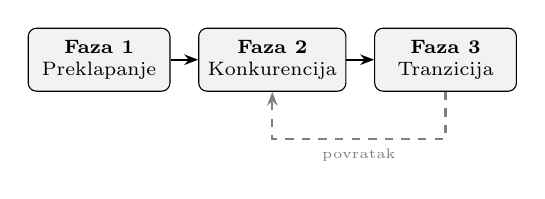
\begin{tikzpicture}[
    phase/.style={draw, rounded corners=3pt, minimum width=1.8cm, minimum height=0.8cm, align=center, font=\scriptsize, fill=black!5},
    arr/.style={-{Stealth[length=5pt]}, thick}
]
\node[phase] (p1) at (0,0) {\textbf{Faza 1}\\Preklapanje};
\node[phase] (p2) at (2.2,0) {\textbf{Faza 2}\\Konkurencija};
\node[phase] (p3) at (4.4,0) {\textbf{Faza 3}\\Tranzicija};

\draw[arr] (p1) -- (p2);
\draw[arr] (p2) -- (p3);
\draw[arr, dashed, gray] (p3.south) -- ++(0,-0.6) -| node[below,font=\tiny,pos=0.25] {povratak} (p2.south);
\end{tikzpicture}
\caption{Trofazna migracija---reverzibilna u svakoj fazi.}
\label{fig:migration}
\end{figure}

Primarni mehanizam pritiska je fiskalni: kada uvjetni porezni obveznici dosegnu ,,ekonomski značajnu manjinu $X$''---skupinu dovoljno veliku da represija protiv nje uzrokuje netrivijalnu ekonomsku štetu i da građanski neposluh postane vjerodostojna prijetnja---država ulazi u pregovore. Za ilustraciju koristimo $X \approx 15\%$ BDP-a, ali stvarni prag ovisi o konkretnom gospodarstvu.

% ============================================================
% 10. SECURITY ANALYSIS
% ============================================================
\section{Sigurnosna analiza}

Razmatramo pet kategorija protivnika: pojedinačne zlonamjerne aktere, organizirane skupine, korporativne protivnike, protivnike na razini države i protivnike na razini protokola.

\textbf{Otpornost na Sybil napade}~\cite{douceur2002}. Izgradnja reputacije zahtijeva dugotrajnu, provjerljivu interakciju. Trošak uspješnog Sybil napada raste linearno s lažnim identitetima i kvadratno s ciljnom razinom reputacije. Rukovanje s više DID-ova paralelno je moguće, ali skupo po dizajnu---svaki identitet mora neovisno akumulirati reputaciju kroz istinsku aktivnost. U slobodnim društvima taj trošak odvraća od površne zlouporabe; u diktaturama, paralelni DID-ovi postaju alat preživljavanja koji omogućuje odjeljivanje otpora, podzemnu koordinaciju i sigurnije snalaženje na crnom tržištu.

\textbf{Obrana od tajnog dogovaranja.} Obrasci uzajamnog podupiranja među zatvorenim skupinama otkrivi su analizom društvenog grafa. Funkcije agregacije reputacije diskontiraju tvrdnje iz čvrsto povezanih izvora.

\textbf{Protivnik na razini države.} Onion usmjeravanje, odsutnost centralizirane infrastrukture i raspodjela uloge Provjeritelja kroz bazu sudionika osiguravaju da potiskivanje zahtijeva mjere nesrazmjerne bilo kojoj koristi.

\textbf{Privatnost nasuprot odgovornosti.} Pseudonimnost---srednji put između anonimnosti i otkrivanja identiteta---omogućuje DID-ovima da akumuliraju smislenu reputaciju bez otkrivanja stvarnog identiteta nositelja.

% ============================================================
% 11. PRIVACY
% ============================================================
\section{Razmatranja o privatnosti}

Model privatnosti RSN-a izgrađen je na pseudonimnosti. Nositelj kontrolira otkrivanje identiteta: minimalno (čisti pseudonim), selektivno (povezane specifične vjerodajnice) ili potpuno (pridružen pravni identitet). Objavljene tvrdnje su trajne---sustav podržava kontekstualni ispravak, ali ne i brisanje. Nositelj može napustiti kompromitirani DID i početi iznova, gubeći akumuliranu reputaciju.

% ============================================================
% 12. RELATED WORK
% ============================================================
\section{Srodni rad}

W3C DID Core specifikacija~\cite{did2022} i Ceramic Network~\cite{ceramic2023} pružaju temelj identiteta. EigenTrust~\cite{kamvar2003} demonstrirao je distribuiranu agregaciju reputacije bez središnjeg autoriteta. SBT-ovi~\cite{weyl2022} uveli su neprenosive društvene tokene. RSN se razlikuje po naglasku na ekonomskom trošku kao filtru kvalitete i po svom mehanizmu za određivanje cijene radikalizma.

DAO-i~\cite{buterin2014} i kvadratno glasovanje~\cite{buterin2019} demonstrirali su izvedivost decentraliziranog upravljanja. RSN izvodi konsenzus iz bilateralnih cjenovnih pregovora, a ne iz glasovanja.

Prijedlog se oslanja na anarho-kapitalističku teoriju~\cite{rothbard1973,hoppe2001} za privatno pružanje usluga, ali odstupa u dva ključna pogleda: dizajniran je za pakost i osvetničke impulse umjesto da pretpostavlja racionalnost, i predlaže postupnu tranziciju umjesto revolucije. Koncept emergentnih društvenih ugovora ima prethodnike u Hayekovoj teoriji spontanog reda~\cite{hayek1973}.

\textbf{Anarho-agorizam.} RSN dijeli značajno zajedničko tlo s agorističkom kontra-ekonomijom~\cite{konkin2006}---posebno naglasak na izgradnji paralelnih institucija i dobrovoljnoj razmjeni. Međutim, agorizam ima tendenciju pretpostavljati racionalan vlastiti interes kao dovoljan mehanizam koordinacije i često mu nedostaje konkretan put migracije od postojećih državnih struktura. RSN eksplicitno ugrađuje neracionalne bihevioralne sklonosti i pruža mehanizam fiskalnog pritiska za postupnu tranziciju.

\textbf{Meritokracija.} RSN može predstavljati prvi funkcionalni opis toga kako meritokracija~\cite{young1958} može nastati kao sistemsko svojstvo, a ne slogan. Tradicionalni meritokratski sustavi zakazuju jer zahtijevaju središnji autoritet da definira i provede ,,zaslugu''. U RSN-u, zasluga proizlazi iz bilateralnih vrednovanja: oni koji isporučuju vrijednost akumuliraju reputaciju; nijedan odbor ne odlučuje tko ima zaslugu.

\textbf{Vlasništvo kao povlastica.} RSN se temeljno razlikuje od anarho-kapitalističkih i austrijskoškolskih tretmana vlasničkih prava kao prirodnih i apsolutnih. U RSN okviru, vlasništvo je \emph{povlastica}---društveno priznanje koje se, u ekstremnim slučajevima, može oduzeti od strane zajednice kada sudionik temeljno prekrši zajedničke norme (izdaja, odbijanje obrane zajednice u egzistencijalnoj krizi, sustavno iskorištavanje). To nije državna eksproprijacija, već povlačenje društvenog priznanja od strane mreže bilateralnih odnosa.

% ============================================================
% 13. LIMITATIONS
% ============================================================
\section{Rasprava i ograničenja}

\textbf{Hladan start.} Vrijednost RSN-a ovisi o mrežnim učincima; rani usvojitelji suočavaju se s ograničenom vrijednošću dok sudjelovanje ne dosegne prag. Međutim, čak i od ranih faza, DID mreža služi kao koristan dopunski izvor informacija. Očekuje se da će se rano vrednovanje reputacije i procjena autoriteta postupno razvijati uz sve veću sofisticiranost.

\textbf{Anti-parazitizam i kontrola pristupa.} Ciljni DID-ovi mogu nametnuti postupne naknade i ograničenja pristupa za upite od DID-ova niske reputacije. To nije binarno, već kontinuirana ljestvica: što manje reputacije DID koji šalje upit ima, to manje informacija dobiva, to duže čeka i to više plaća. Taj mehanizam potiče istinsko sudjelovanje umjesto pasivne konzumacije.

\textbf{Nejednakost pristupa.} Trošak objavljivanja tvrdnji može filtrirati legitimne pritužbe ekonomski slabijih sudionika. Ublažavanje: svaki sudionik istodobno služi kao potencijalni provjeritelj (ili delegira tu ulogu) i zarađuje naknade za provjeru. Kroz dovoljan vremenski horizont, neradikalan sudionik trebao bi se približiti financijskoj neutralnosti---prihod od provjere približno kompenzira troškove objavljivanja. To je statističko očekivanje, a ne jamstvo.

\textbf{Nejednakost reputacije.} Rani usvojitelji akumuliraju prednosti koje mogu stvoriti prepreke za one koji dolaze kasnije. Međutim, vrednovanje reputacije provode neovisni pružatelji koji mogu odabrati ublažiti prednost prvog poteza kroz svoje algoritme agregacije. Biti prvi s dobrom reputacijom legitimna je usporedna ekonomska prednost---i to je po dizajnu.

\textbf{Otvorena pitanja.} Optimalne funkcije troška, standardi agregacije, upravljanje protokolom i interakcija s reputacijskim podacima koje sintetizira umjetna inteligencija ostaju područja za budući rad.

Ovaj rad ne tvrdi da će RSN proizvesti optimalne ishode u svim okolnostima. On tvrdi da RSN predstavlja \emph{izvedivu} alternativu---tehnički provedivu, ekonomski samoodrživu i društveno kompatibilnu s ljudskim bihevioralnim sklonostima kakve one stvarno jesu.

% ============================================================
% 14. CONCLUSION
% ============================================================
\section{Zaključak}

Ovaj rad predstavio je Reputacijsku društvenu mrežu, decentralizirani protokol koji omogućuje pseudonimnu, provjerljivu razmjenu reputacije. Načelo skupog radikalizma osigurava da se prijevarne tvrdnje isključe cijenom bez cenzure. Predloženi put migracije omogućuje postupnu, reverzibilnu tranziciju od postojećih institucija. Dizajn ugrađuje ljudsku prirodu kakva jest---uključujući sitničavost, pakost i želju za osvetničkim zadovoljstvom---umjesto da zahtijeva ideološku transformaciju. Rezultat nije utopija, već sustav u kojem je pravda dostupna, reputacija se zarađuje, a trošak nedoličnog ponašanja snosi strana koja ga je uzrokovala.

% ============================================================
% REFERENCES
% ============================================================
\bibliography{references}

\end{document}
